\documentclass[12pt, a4paper]{extarticle}


% Russian text support
\usepackage[T2A]{fontenc}
\usepackage[utf8]{inputenc}
\usepackage[russian]{babel}

% Some useful packages
\usepackage{indentfirst}
\usepackage{etoolbox}
\usepackage{amsmath}
\usepackage{amssymb}
\usepackage{amsfonts}
\usepackage{tabularx}

% Pictures support
\usepackage{graphicx}
\graphicspath{ {./images/} }

% Page geometry
\usepackage[
    left=3cm,
    right=1cm,
    top=2cm,
    bottom=2cm
]{geometry}

% Code
\usepackage{listings}
\usepackage{xcolor}

\definecolor{codegreen}{rgb}{0,0.6,0}
\definecolor{codegray}{rgb}{0.5,0.5,0.5}
\definecolor{codepurple}{rgb}{0.58,0,0.82}
\definecolor{backcolour}{rgb}{1,1,1}

\lstdefinestyle{codestyle}{
    backgroundcolor=\color{backcolour},   
    commentstyle=\color{codegreen},
    keywordstyle=\color{magenta},
    numberstyle=\tiny\color{codegray},
    stringstyle=\color{codepurple},
    basicstyle=\ttfamily\footnotesize,
    breakatwhitespace=false,         
    breaklines=true,                 
    captionpos=b,                    
    keepspaces=true,                 
    numbers=left,                    
    numbersep=5pt,                  
    showspaces=false,                
    showstringspaces=false,
    showtabs=false,                  
    tabsize=2,
    extendedchars=\true,
}

\lstset{style=codestyle}

% Make titles not to have numbering
\newenvironment*{dummyenv}{}{}

\newcommand{\mysection}[1]{
    \addcontentsline{toc}{section}{#1}
    \begin{dummyenv}
        \bfseries\large #1
    \end{dummyenv}
}

\makeatletter
\patchcmd{\l@section}
  {\hfil}
  {\leaders\hbox{\normalfont$\m@th\mkern \@dotsep mu\hbox{.}\mkern \@dotsep mu$}\hfill}
  {}{}
\makeatother

% Some useful stuff
\newcommand{\Answer}[1]{\textbf{Ответ:} #1}

\renewcommand{\Pr}[1]{\text{Pr}\left[ #1 \right]}

\newcolumntype{Y}{>{\centering\arraybackslash}X}

% Here we go...
\title{БДЗ по прикладной криптографии}
\author{Фирсов Георгий, М21-507}

\begin{document}

\maketitle

\tableofcontents

\pagebreak
\mysection{Задание 1}

При известном заранее значении $D$ нарушитель может единожды найти такое значение $z$, что:
\begin{equation}
    \texttt{SHA256}(z) < \frac{2 ^ n}{D}.
\end{equation}

Это потребует некоторого времени, но идея в том, что это делается единожды и заранее.

Далее при обнародовании $x$ нарушитель вычисляет $y = z \oplus x$. При этом верна следующая
цепочка:
\begin{equation}
    H(x, y) = H(x, x \oplus z) = \texttt{SHA256}(x \oplus x \oplus z) = 
        \texttt{SHA256}(z) < \frac{2 ^ n}{D},
\end{equation}
то есть нарушитель может для каждого $x$ найти такой $y$, что $H(x, y) < \frac{2 ^ n}{D}$
за некоторое константное время.
\\

\mysection{Задание 2}

\begin{enumerate}
    \item На рисунке \ref{fig:2.1} представлен процесс вычисления хэша $R_i$ (или просто искомого
        коммитмента $S$), входящего в заголовок $i$-го блока, при помощи троичного дерева Меркла. 
        Фактически это достаточно очевидное само по себе переложение процесса вычисления на 
        троичное дерево вместо двоичного.
        \begin{figure}[h!]
            \centering
            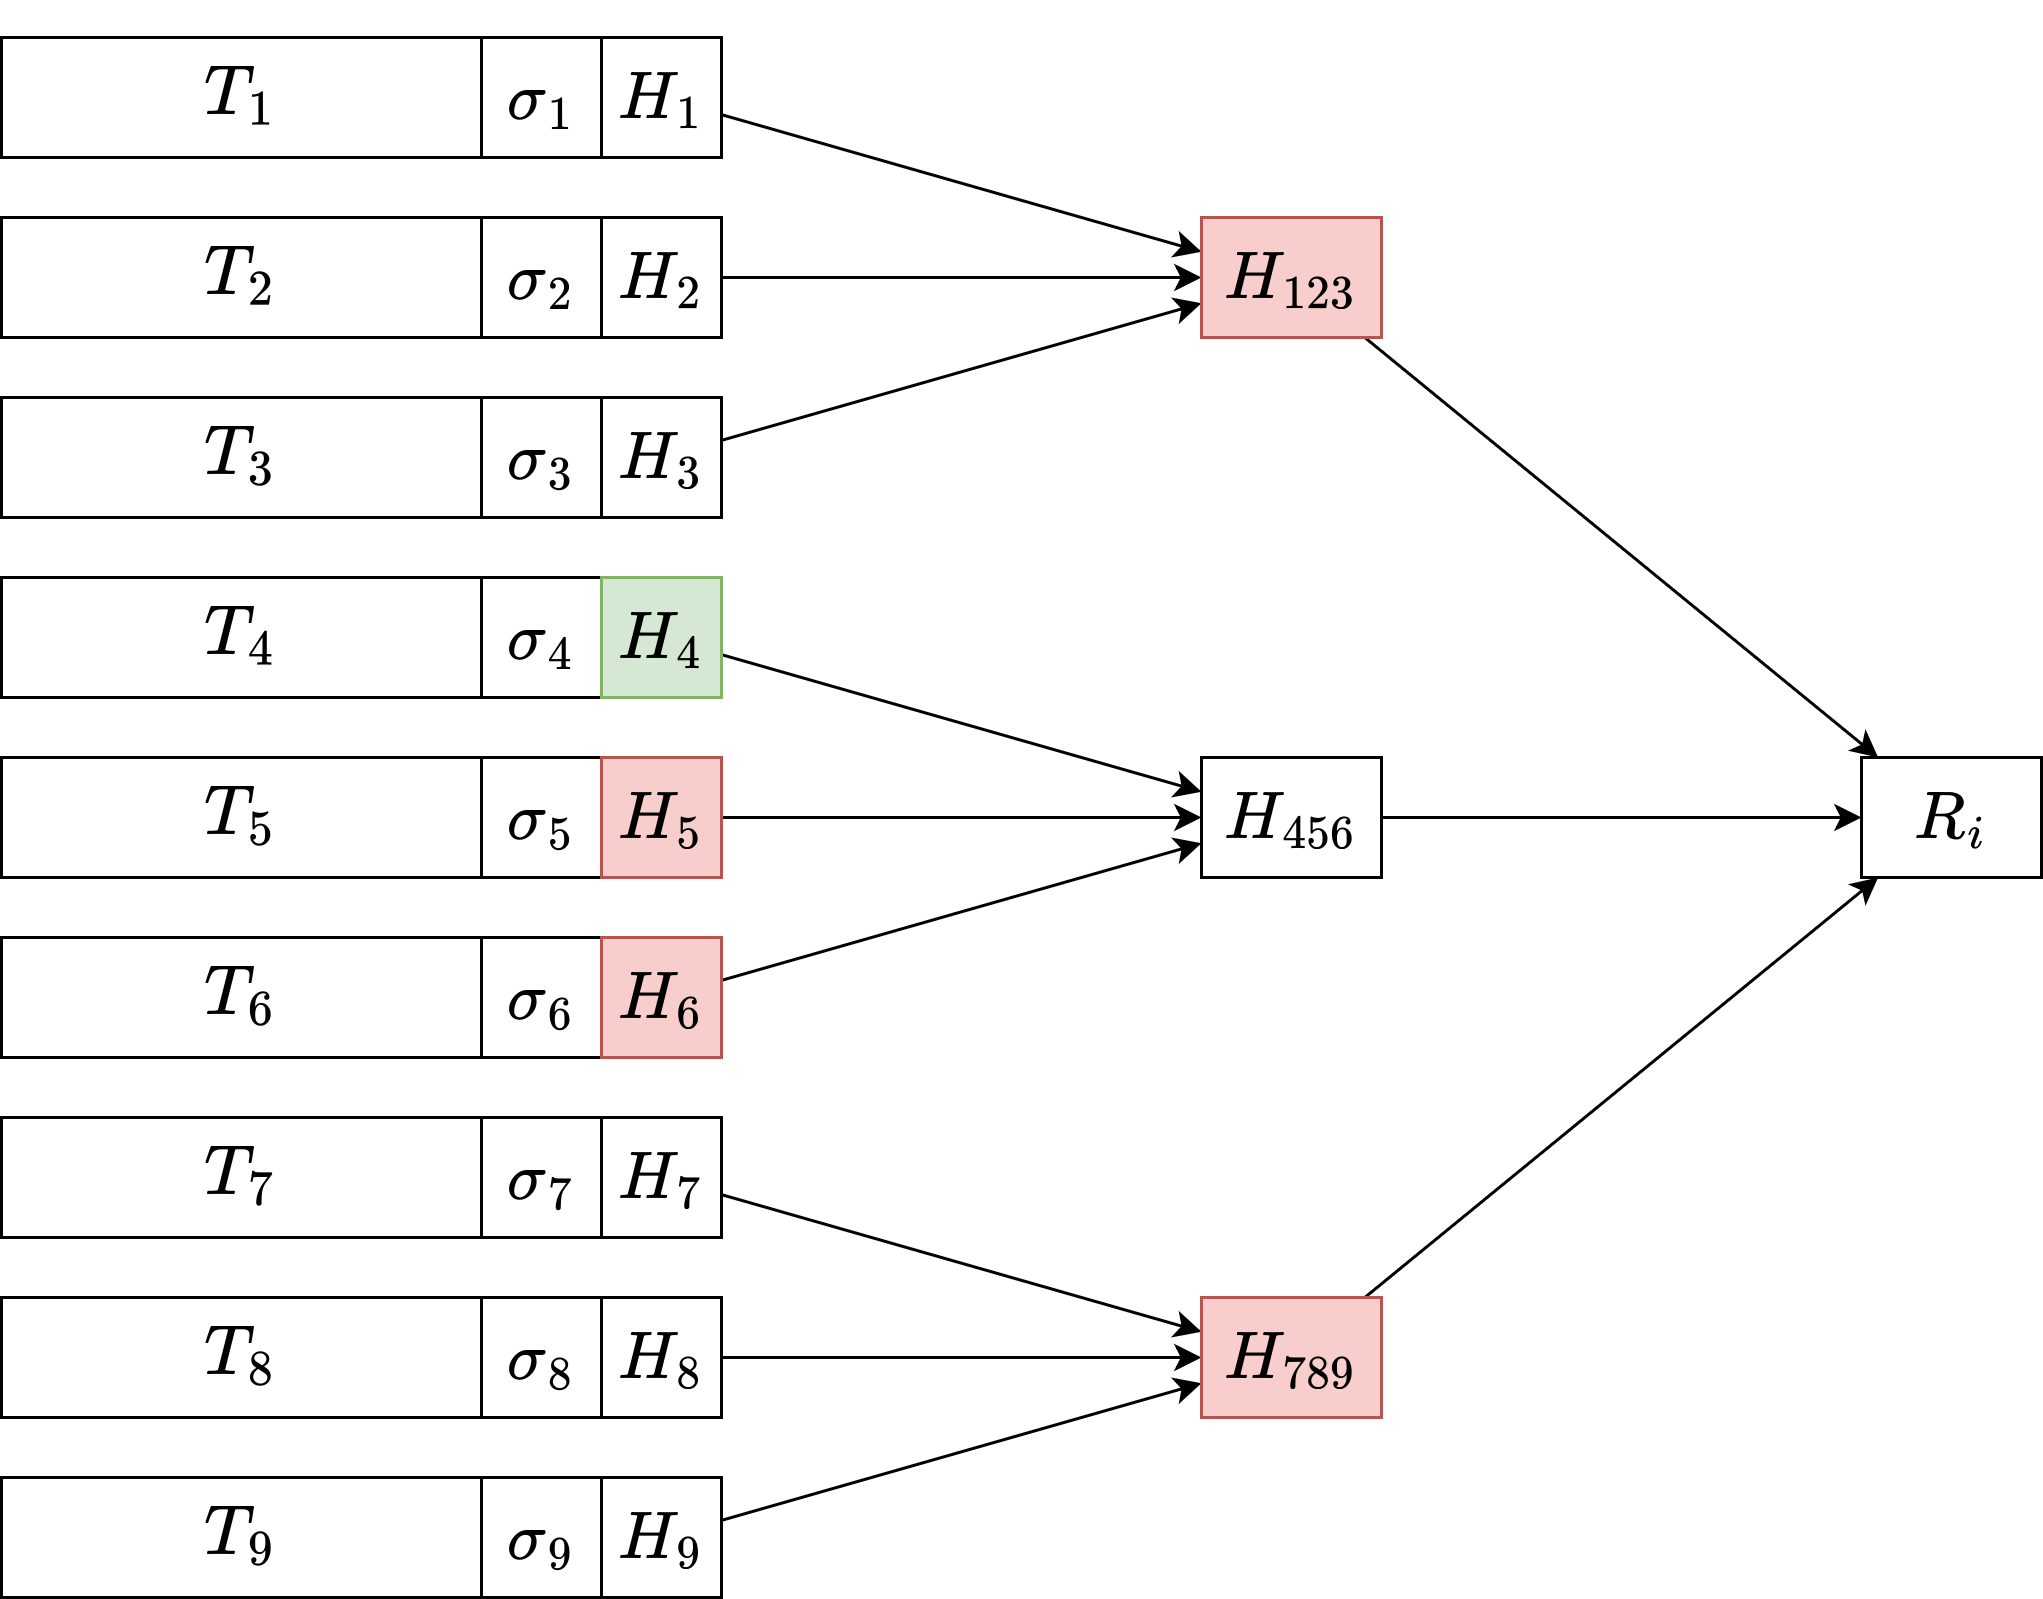
\includegraphics[width=\textwidth]{2.1.png}
            \caption{Схема вычисления хэша при помощи троичного дерева Меркла}
            \label{fig:2.1}
        \end{figure}
        
        Для того, чтобы доказать вхождение транзакции $T_4$ (хэш которой выделен зеленым на рисунке
        \ref{fig:2.1}) требуется предоставить Борису следующие значения: $H_5$, $H_6$ (соседние
        хэши) и $H_{123}$, $H_{789}$ (хэши соседних поддеревьев). Данные значения на рисунке
        \ref{fig:2.1} выделены красным.
        
        Борис вычисляет $\tilde{H}_{456}$ на основе известного $H_4$ и предоставленных $H_5$, $H_6$
        ($\tilde{H}_{456} = H(H_4 || H_5 || H_6)$), после чего на основе полученного значения и
        предоставленных $H_{123}$, $H_{789}$ рассчитывает $\tilde{S} = H(H_{123} || \tilde{H}_{456}
        || H_{789})$. Если $\tilde{S} = R_i$, то $T_4$ содержится в блоке (при условии, что все 
        предоставленные хэши верны, что было бы логично при доказательстве).
        
    \item Отметим, что путь от корня до проверяемой вершины содержит $\lceil \log_k n \rceil$
        элементов дерева. Для каждого элемента необходимо предоставить $k - 1$ хэш --- это
        хэши соседних поддеревьев (а для листового уровня --- соседние хэши-листы). Таким
        образом получается следующая формула для длины доказательства: 
        \begin{equation}
            (k - 1) \cdot \lceil \log_k n \rceil.
        \end{equation}
        
        \Answer{$(k - 1) \cdot \lceil \log_k n \rceil$}.
        
    \item Ясно, что для $x > 1$ выполнено: $\log_2 x < 2 \cdot \log_3 x$. Более наглядно это
        представлено на рисунке \ref{fig:2.3}:
        \begin{figure}[h!]
            \centering
            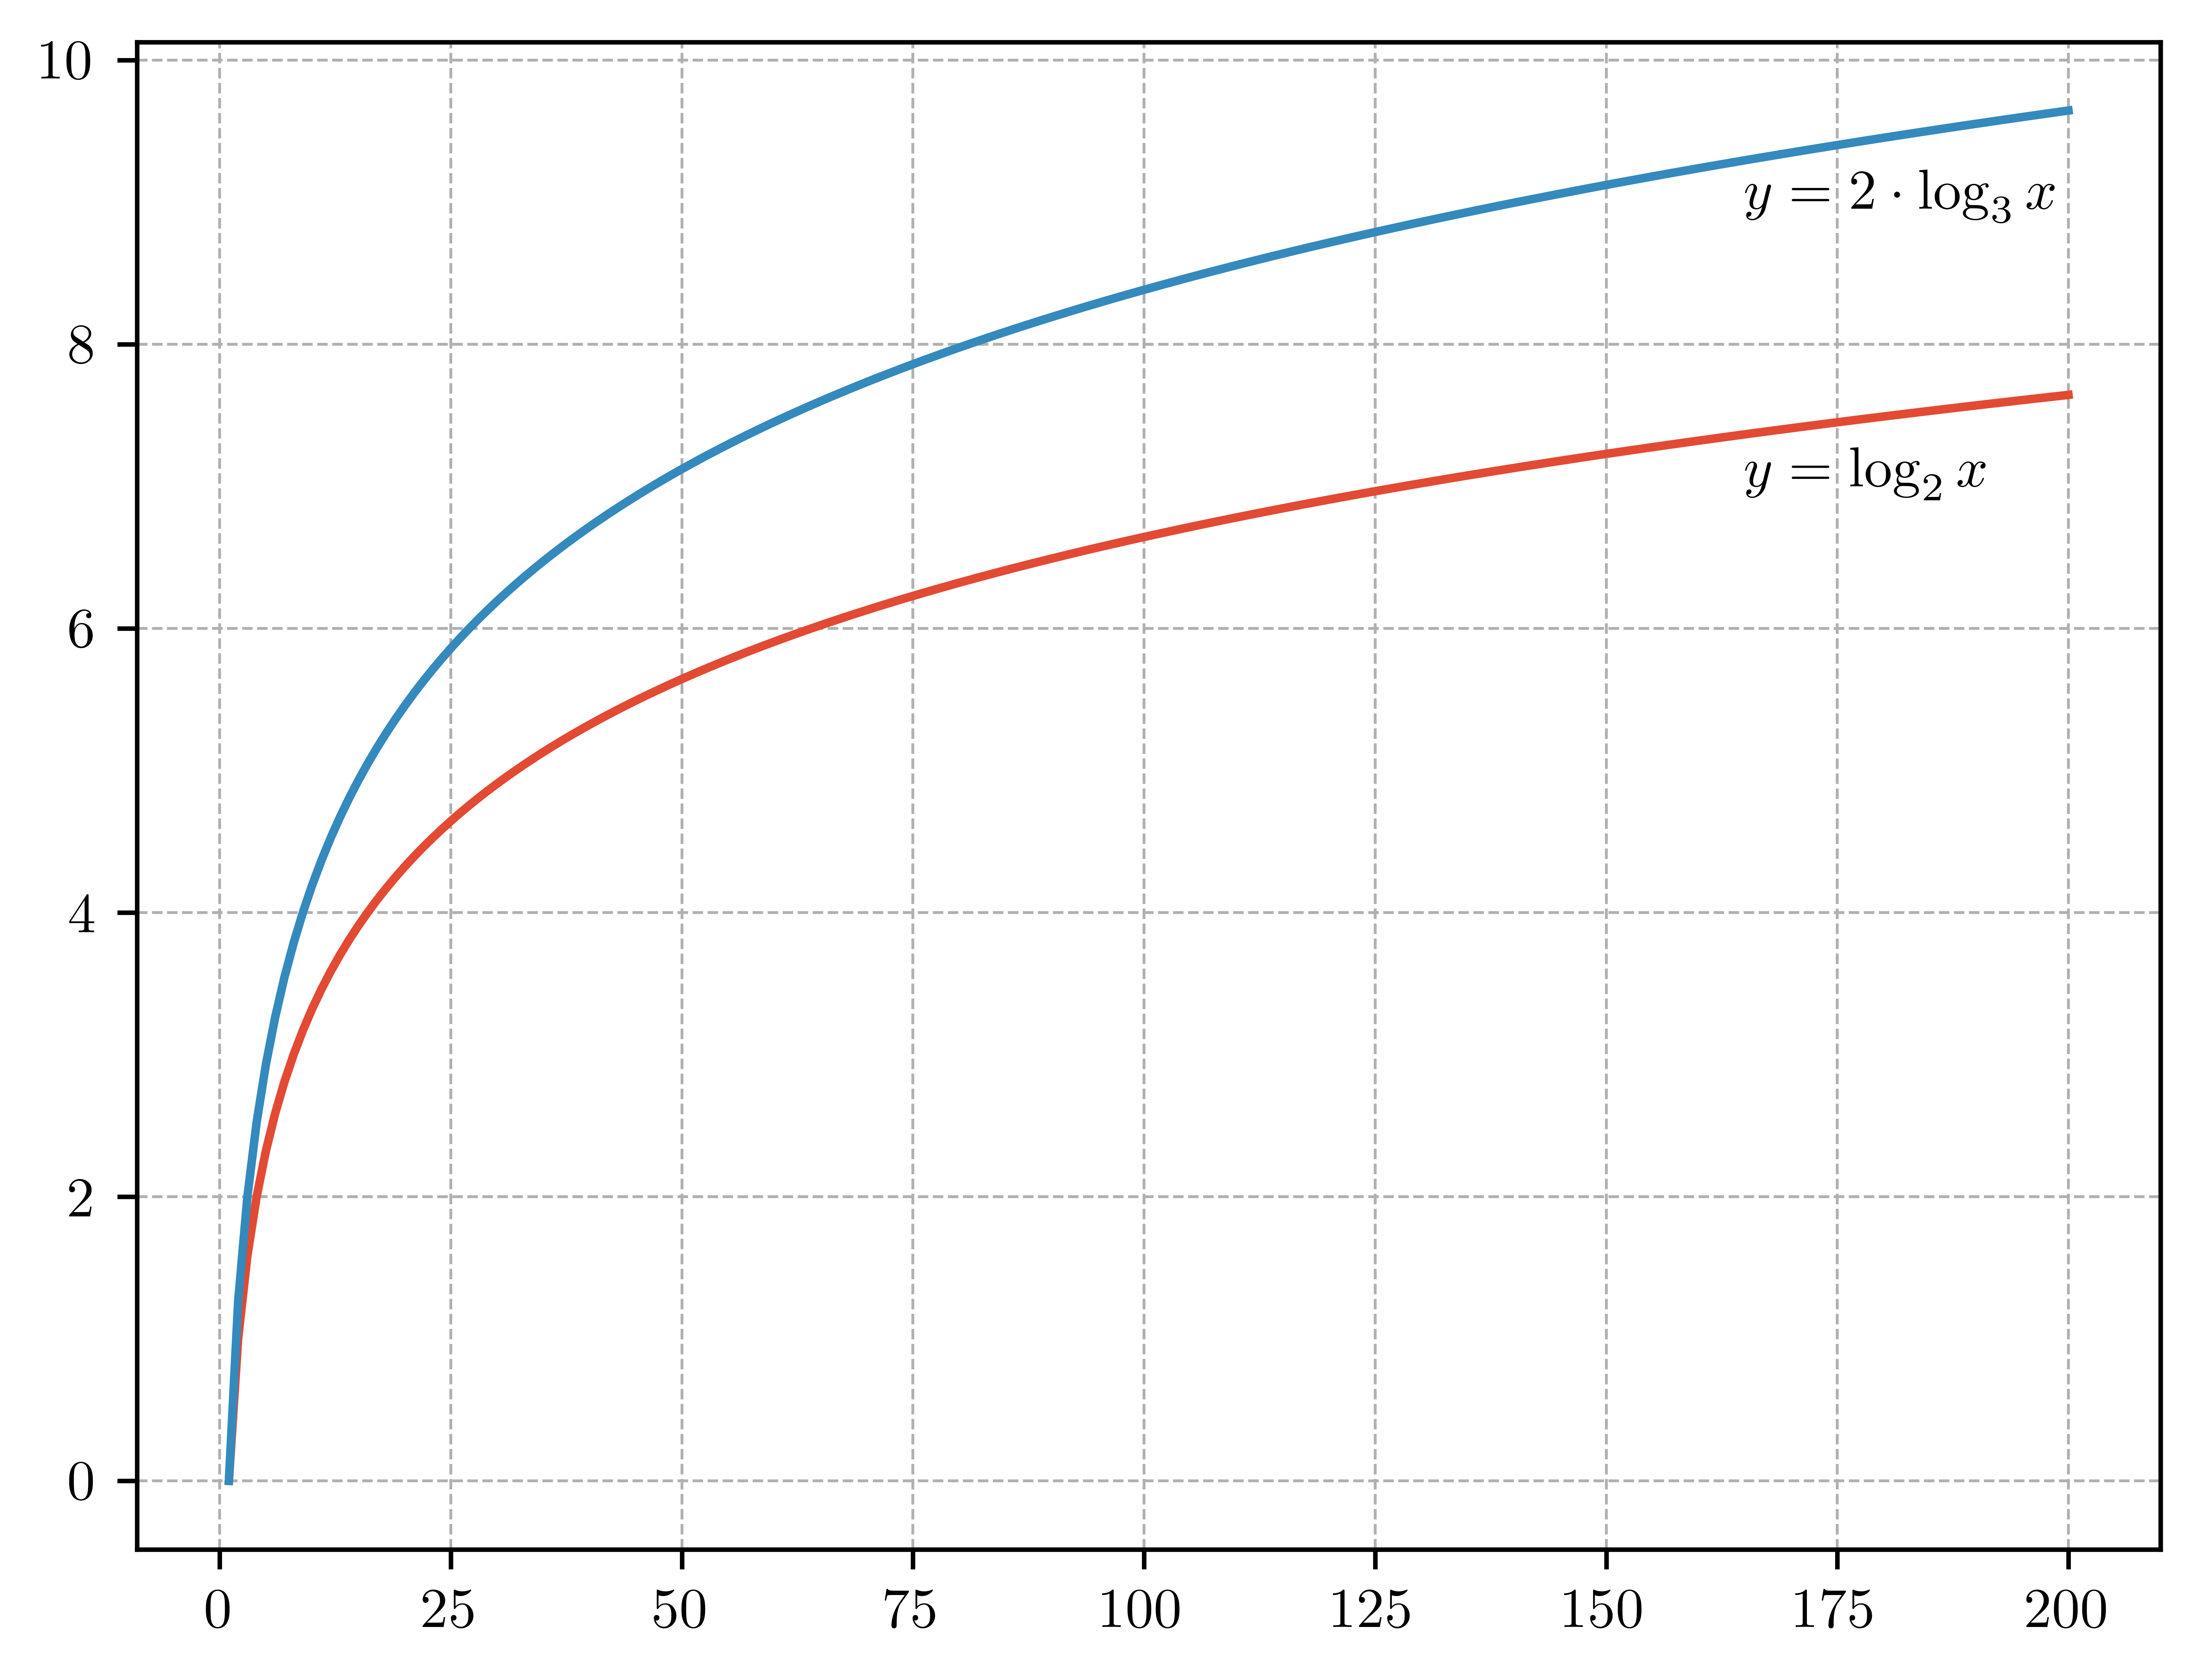
\includegraphics[width=0.7\textwidth]{2.3.png}
            \caption{графики двоичного (красная линия) и удвоенного троичного (синяя линия) 
                логарифмов в одинаковом масштабе}
            \label{fig:2.3}
        \end{figure}
        
        Из этого следует, что использование двоичного дерева Меркла эффективнее, чем троичного (и на 
        самом деле какого-бы то ни было еще), так как длина доказательства для него будет меньше.
        
        \Answer{двоичное дерево использовать оптимальнее, чем троичное}.
\end{enumerate}

\mysection{Задание 3}

Все пункты данной задачи будут для наглядности проиллюстрированы конкретным примером, на основе
которого далее будет дано обобщенное решение.

\begin{enumerate}
    \item На рисунке \ref{fig:3.1} изображена цепочка блоков: зеленым выделен блок, заголовок которого
        хранится в памяти компьютера Бориса, желтым --- блок, в который входит транзакция, для которой
        требуется доказать вхождение в цепь. Через $R_i$ обозначается хэш-вершина дерева Меркла для 
        транзакций $i$-го блока, через $H_{i - 1}$ --- хэш заголовка предыдущего (то есть с индексом 
        $i - 1$) блока.
        \begin{figure}[h!]
            \centering
            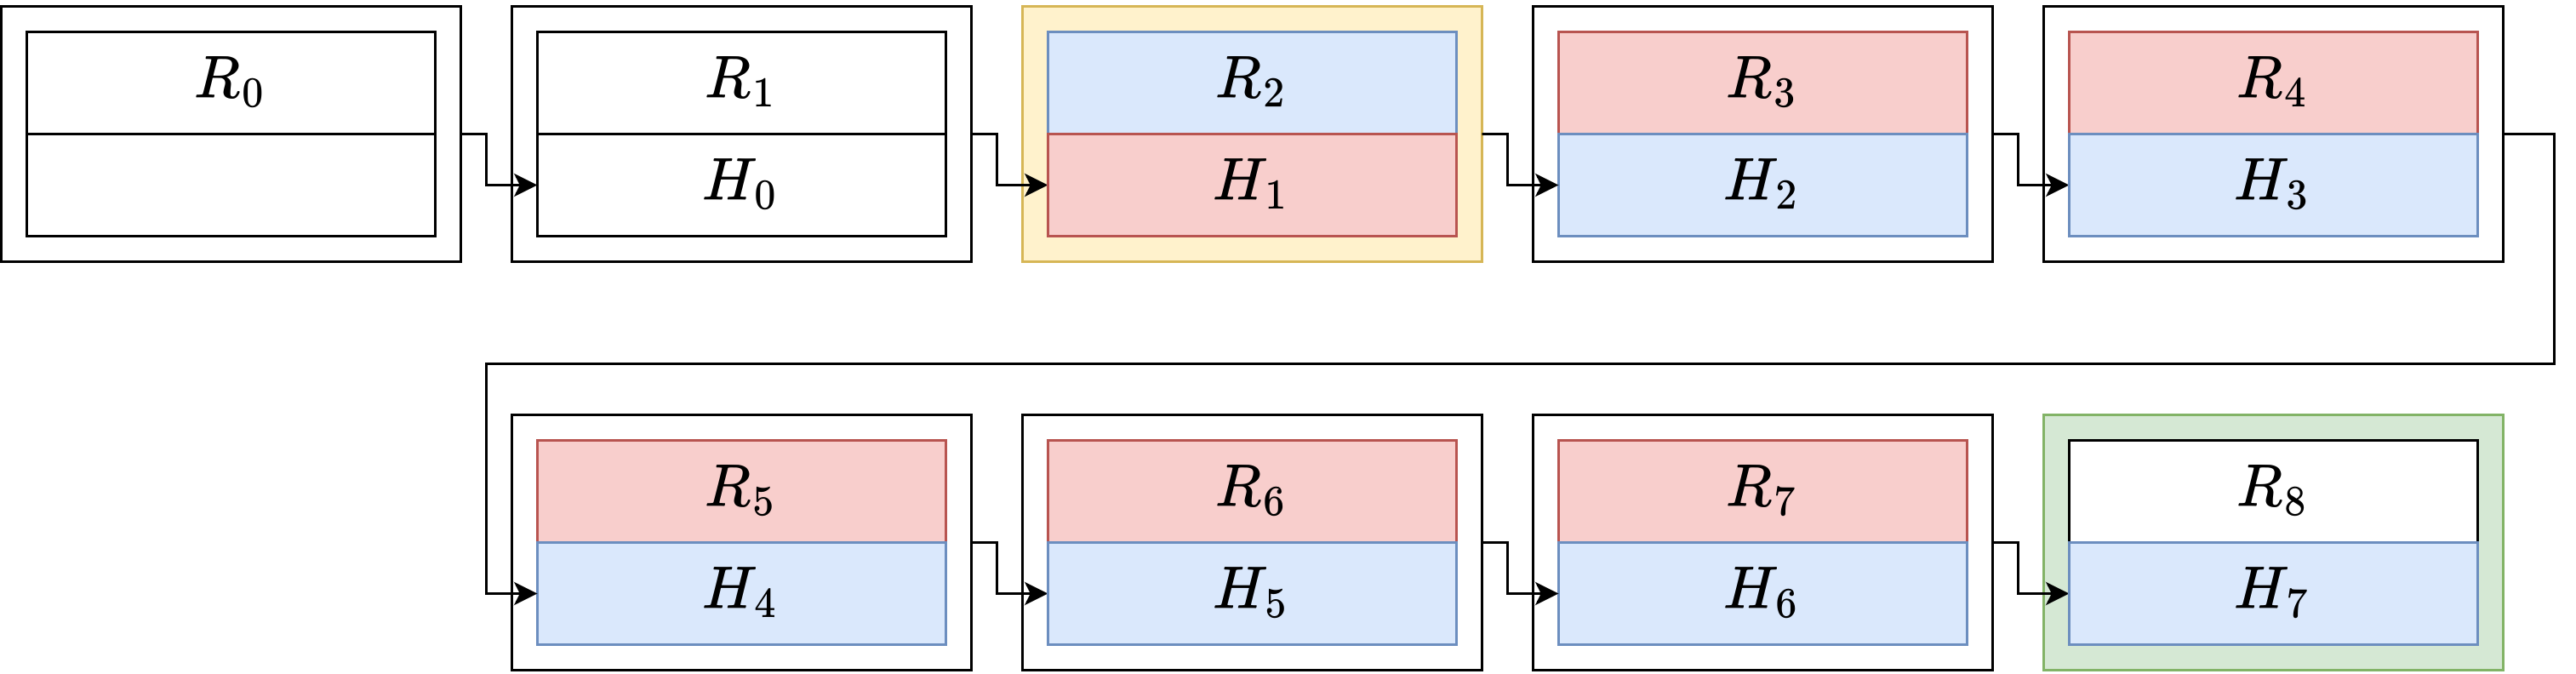
\includegraphics[width=\textwidth]{3.1.png}
            \caption{Доказательство нахождения транзакции из блока с индексом 2 в цепи}
            \label{fig:3.1}
        \end{figure}
        
        Красным цветом на рисунке \ref{fig:3.1} обозначаются данные, которые предоставляются Анной
        для доказательства, синим --- вычисляемые Борисом значения. Следует отметить, что для вычисления
        значения $R_2$ (в изображенном примере) Борису требуется получить от Анны еще 
        $\lceil \log_2 n \rceil$ хэшей для дерева Меркла (см. задачу 2). Проведем обобщение.
        
        \Answer{Анне требуется предоставить Борису следующие данные:
            \begin{itemize}
                \item $\lceil \log_2 n \rceil$ хэшей для дерева Меркла для вычисления хэша $R_i$,
                    где $i$ --- индекс блока, в который входит исследуемая транзакция;
                \item хэш заголовка предыдущего блока $H_{i - 1}$, на основе которого в совокупности с 
                    рассчитанным $R_i$ вычисляется $H_i$;
                \item хэши-вершины деревьев Меркла для блоков от $i + 1$ до $c - 1$, где $c$ --- индекс
                    <<текущего>> блока.
            \end{itemize}
        }
        
    \item Для иллюстрации данного пункта будет использоваться рисунок \ref{fig:3.1}. В этом случае $k = 6$
        (то есть прямо как и в условии). Размер хэша $32$ байта (это 256 бит SHA256). Как было сказано
        в предыдущем пункте, требуется передать:
        \begin{itemize}
            \item $\lceil \log_2 n \rceil$ хэшей для дерева Меркла: $\lceil \log_2 1024 \rceil \cdot 
                32 = 320$ байт;
            \item хэш заголовка предыдущего блока: $32$ байта;
            \item $k - 1$ хэшей-вершин деревьев Меркла блоков между блоком с транзакцией и головным:
                $(6 - 1) \cdot 32 = 160$ байт.
        \end{itemize}
        
        Итоговая формула: $\left(\lceil \log_2 n \rceil + k\right) h$, где $h$ --- размер хэша.
        
        \Answer{$320 + 32 + 160 = 512$ байт. Формулу для расчета см. выше.}
    
    \item Оптимизация происходит за счет того, что при доказательстве можно пропустить проверку
        некоторых промежуточных блоков. Пример ускорения показан на рисунке \ref{fig:3.3} для двух
        случаев: когда текущий блок у Бориса имеет индекс 8 и 9. Красной линией показан <<обходной>>
        путь, позволяющий не проверять промежуточные блоки. Так, в первом случае достаточно предоставить
        только хэши для проверки дерева Меркла генезис-блока, на основе вычисленного значения вершины
        которого вычисляется хэш заголовка $H_0$. Во втором случае текущий блок чуть дальше, а поэтому
        требуется дополнительно предоставить хэш $H_7$ и хэш-вершину дерева Меркла для предыдущего 
        блока $R_8$. При этом данные случаи являются в некотором смысле одними из самых оптимальных.
        \begin{figure}[h!]
            \centering
            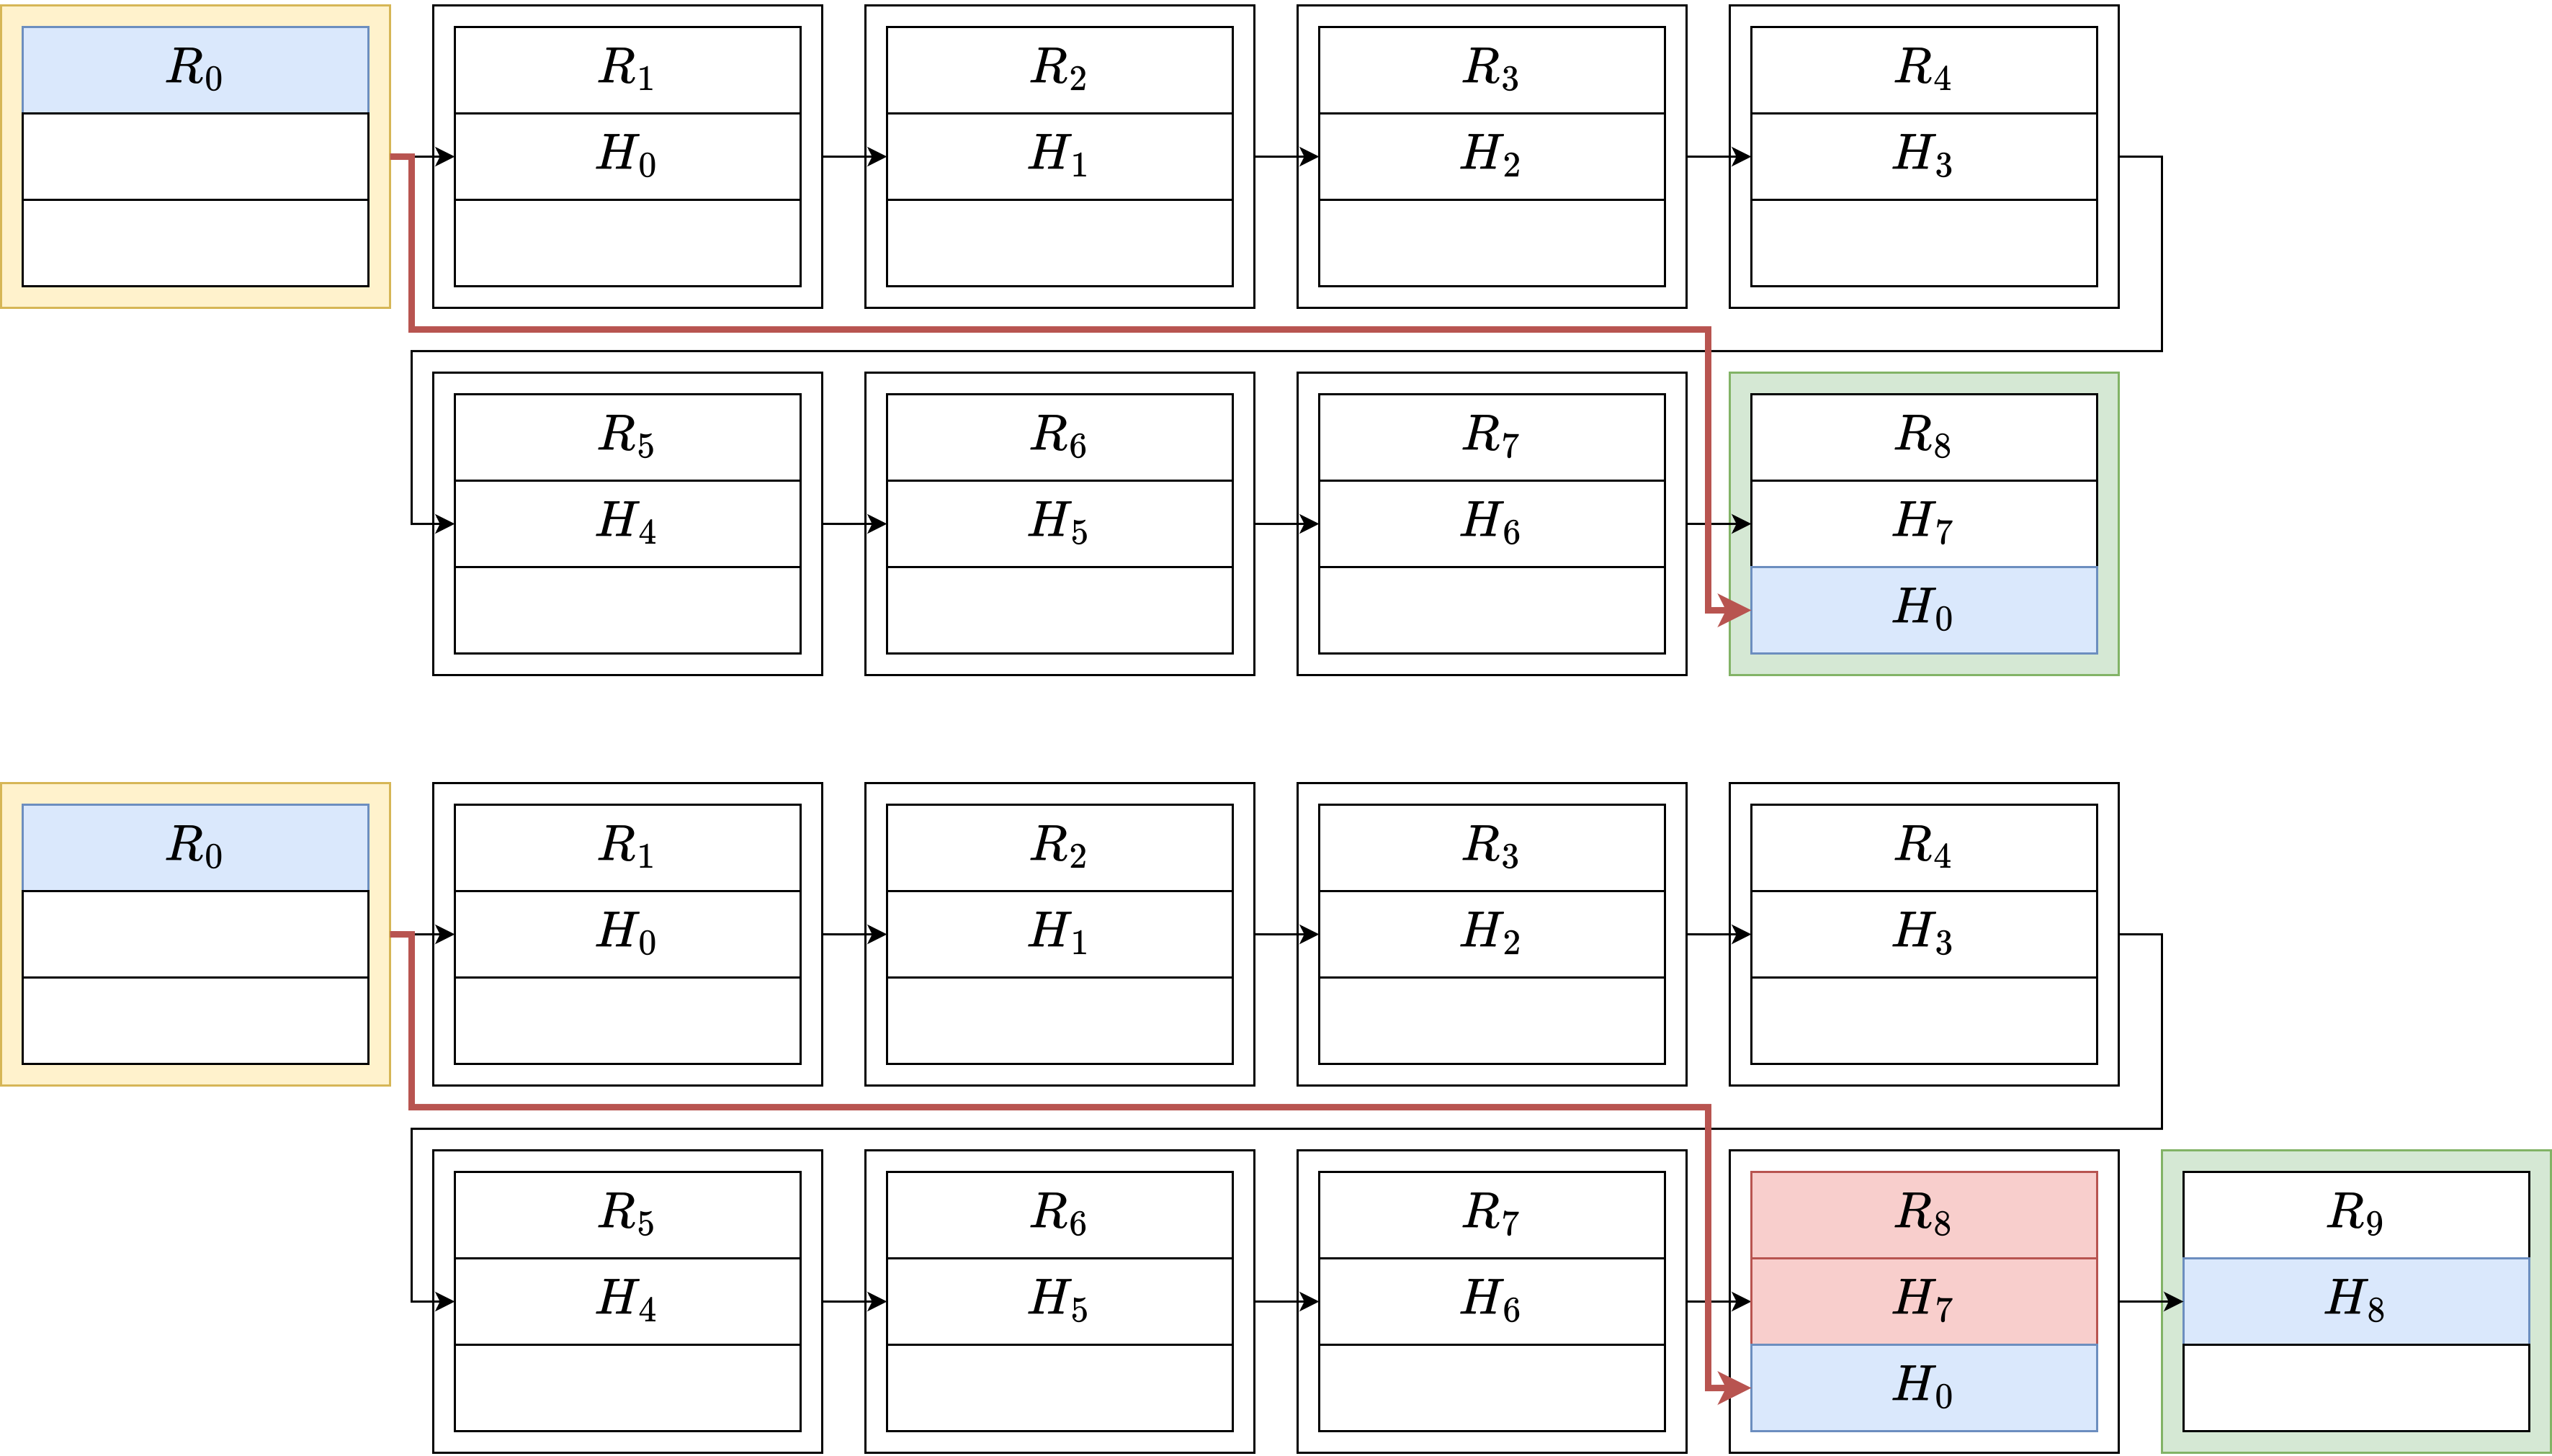
\includegraphics[width=\textwidth]{3.3.png}
            \caption{Пример оптимизации доказательства при помощи рассматриваемой схемы}
            \label{fig:3.3}
        \end{figure}
        
        Рассмотрим теперь худший случай: доказательство вхождения транзакции из блока с индексом 1
        при индексе текущего $k = 2 ^ d - 1$ для $d \in \mathbb{N}$. Рассмотрим пример <<пути>>
        проведения доказательства на более высоком уровне абстракции (рис. \ref{fig:3.3-2}). Красным
        цветом обозначены <<обходные>> пути.
        \begin{figure}[h!]
            \centering
            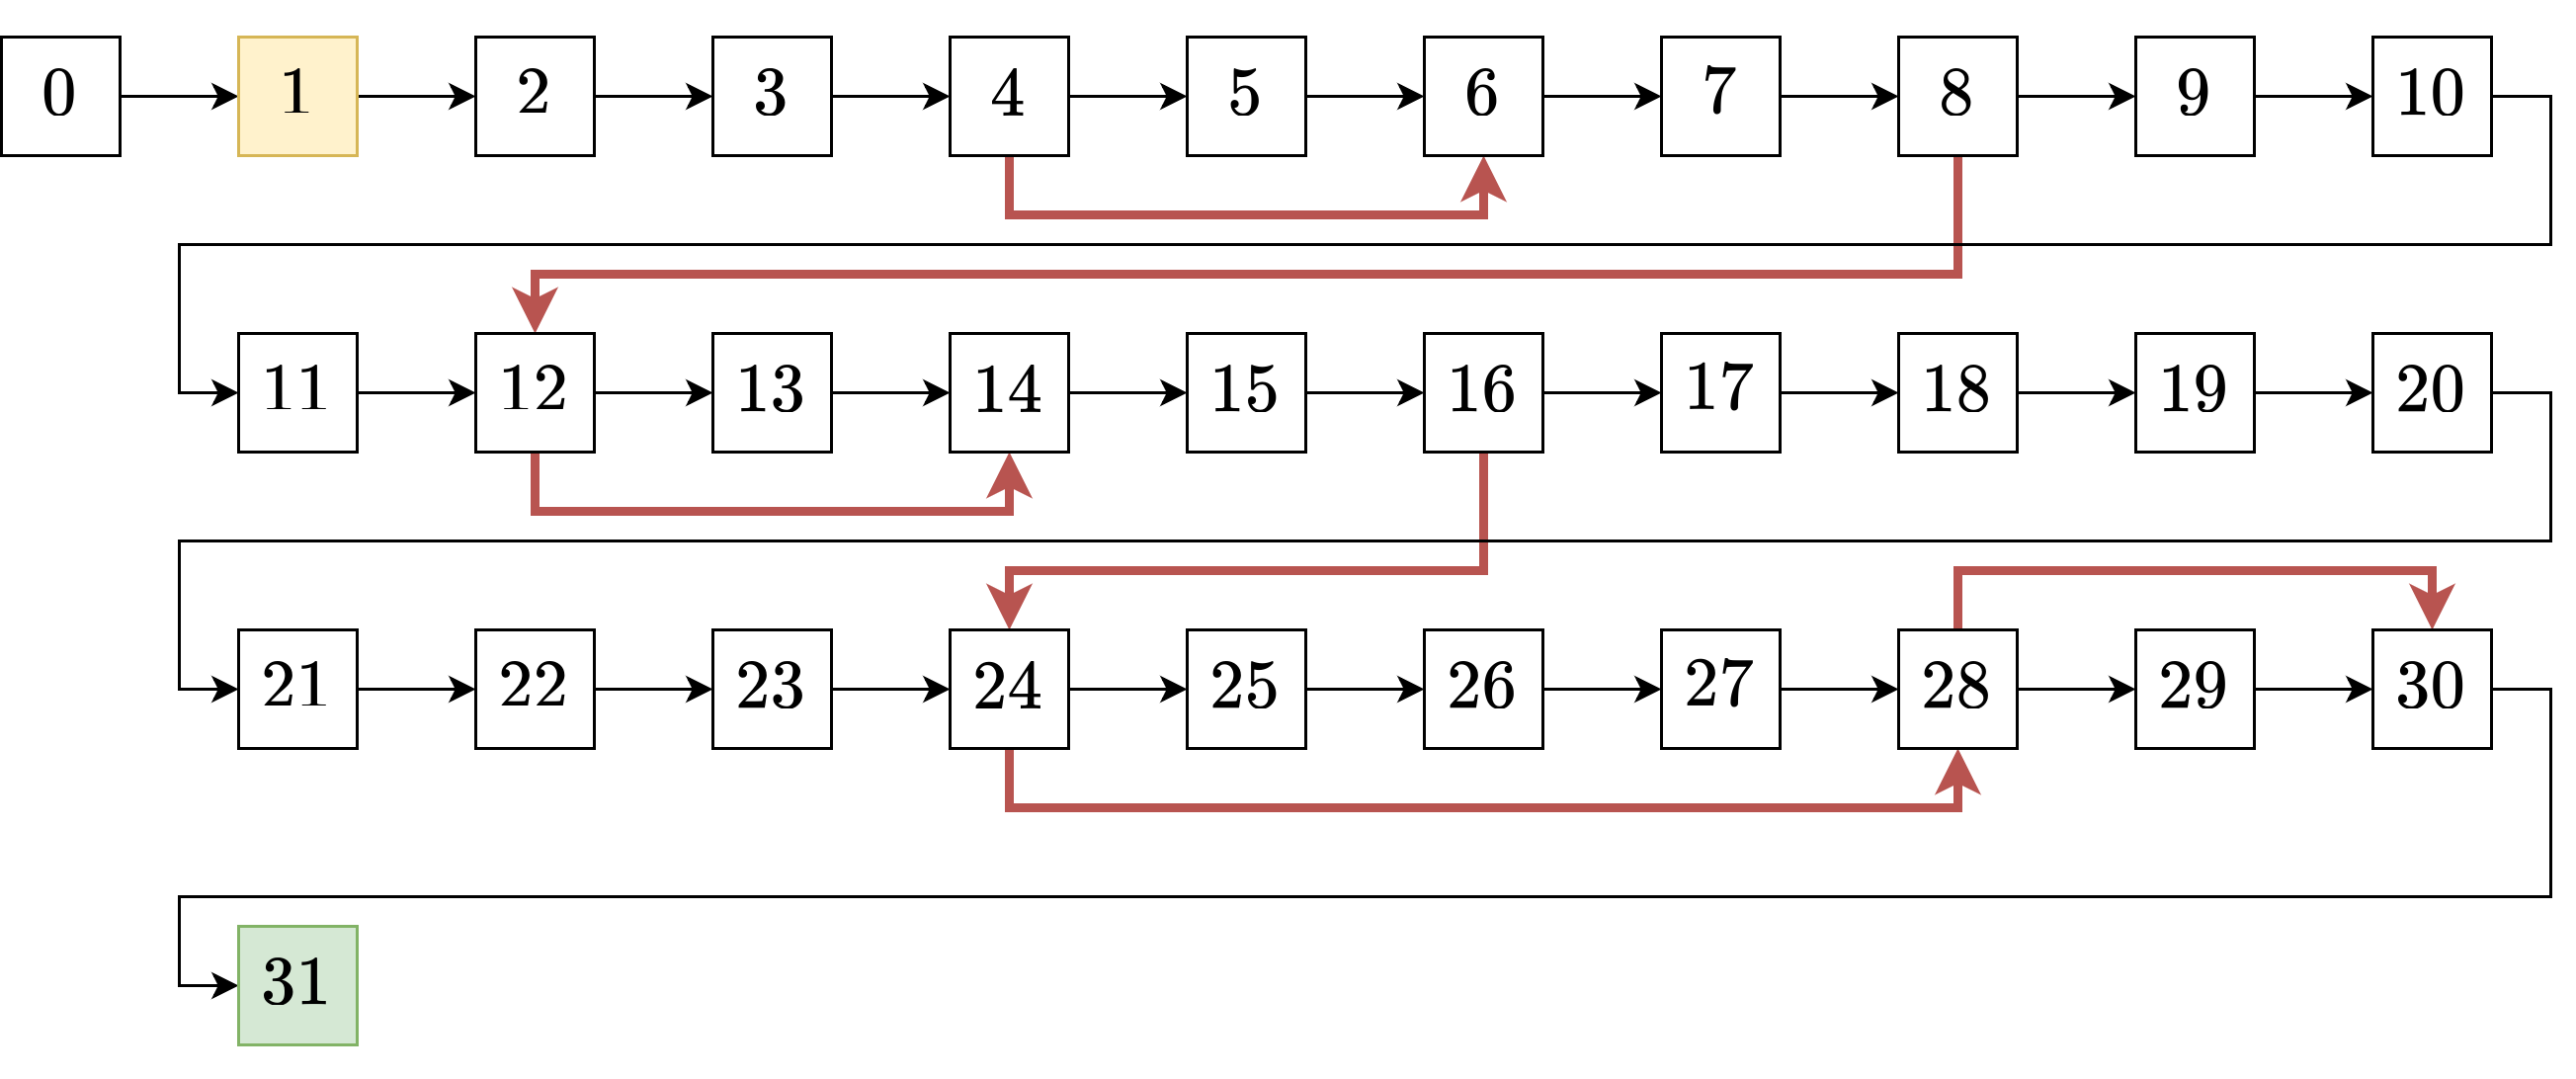
\includegraphics[width=\textwidth]{3.3-2.png}
            \caption{Пример <<худшего>> случая доказательства при помощи рассматриваемой схемы для $k = 31$}
            \label{fig:3.3-2}
        \end{figure}
        
        Как видно из рисунков \ref{fig:3.1} и \ref{fig:3.3}, один <<обычный>> переход <<стоит>> 1 хэш (только
        хэш-вершина дерева Меркла для блока, в который осуществляется переход), а <<обходной>> путь --- 2 хэша
        (тот же хэш-вершина дерева Меркла, а также хэш заголовка блока, который предшествует тому, в который
        осуществляется переход). Таким образом, полный объем доказательства составляет:
        \begin{equation}
            \mathfrak{v}(n, k) = \lceil \log_2 n \rceil + 2 \cdot \mathfrak{l}(k) + \mathfrak{s}(k),
        \end{equation}
        где $\mathfrak{l}(k)$ --- количество <<обходных>> переходов, $\mathfrak{s}(k)$ --- количество
        <<обычных>> переходов. При этом хэш заголовка генезис-блока уже учтен в данной формуле, так как
        переход от 1-го блока ко 2-му как раз ему и соответствует (в остальных случаях переход соответствует,
        как и было сказано, хэшу-вершине дерева Меркла).
        
        В приложении А предоставлен код, который для входного параметра $k$ возвращает количество 
        <<обходных>> путей, количество <<обычных>> путей (то есть путей в следующий блок) и список блоков, 
        для которых требуется доказательство правильности хэша.
        
        В таблице \ref{tbl:3.3} представлены результаты работы функции \texttt{get\_path} из приложенного
        листинга для $d = \overline{2, 15}$.
        \begin{table}[h!]
            \caption{Значения $\mathfrak{l}(k)$ и $\mathfrak{s}(k)$ для значений $k = 2 ^ d - 1$
                для последовательных значений $d = \overline{2, 15}$}
            \label{tbl:3.3}
            \begin{tabularx}{\textwidth}{|Y|Y|Y|Y|}
                \hline
                 $d$ &     $k$ & $\mathfrak{l}(k)$ & $\mathfrak{s}(k)$ \\
                \hline
                 $2$ &     $3$ &               $0$ &               $2$ \\
                \hline
                 $3$ &     $7$ &               $1$ &               $4$ \\
                \hline
                 $4$ &    $15$ &               $3$ &               $6$ \\
                \hline
                 $5$ &    $31$ &               $6$ &               $8$ \\
                \hline
                 $6$ &    $63$ &              $10$ &              $10$ \\
                \hline
                 $7$ &   $127$ &              $15$ &              $12$ \\
                \hline
                 $8$ &   $255$ &              $21$ &              $14$ \\
                \hline
                 $9$ &   $511$ &              $28$ &              $16$ \\
                \hline
                $10$ &  $1023$ &              $36$ &              $18$ \\
                \hline
                $11$ &  $2047$ &              $45$ &              $20$ \\
                \hline
                $12$ &  $4095$ &              $55$ &              $22$ \\
                \hline
                $13$ &  $8191$ &              $66$ &              $24$ \\
                \hline
                $14$ & $16383$ &              $78$ &              $25$ \\
                \hline
                $15$ & $32767$ &              $91$ &              $26$ \\
                \hline
            \end{tabularx}
        \end{table}
        
        Обозначим: $l_{d} = \mathfrak{l}(k)$, $s_d = \mathfrak{s}(k)$, где $d = \log_2(k + 1)$ и 
        заметим следующее:
        \begin{equation}
        \begin{split}
            & l_d = l_{d - 1} + (d - 2), l_2 = 0 \\
            & s_d = 2 \cdot (d - 1).
        \end{split}
        \end{equation}
        
        Далее получим явное выражение для $l_d$:
        \begin{equation}
        \begin{split}
            l_d & = l_{d - 2} + (d - 3) + (d - 2) = ... = l_2 + 1 + ... + (d - 3) + (d - 2) = \\
            & = \sum_{j = 0}^{d - 2} j = \frac{(d - 2)(d - 1)}{2}.
        \end{split}
        \end{equation}
        
        Тогда:
        \begin{equation}
        \begin{split}
            \mathfrak{v}(n, k) & = \lceil \log_2 n \rceil + 2 \cdot \frac{(d - 2)(d - 1)}{2} + 
                2 \cdot (d - 1) = \\
            & = \lceil \log_2 n \rceil + d (d - 1).
        \end{split}
        \end{equation}
        
        \Answer{$\mathfrak{v}(n, k) = \lceil \log_2 n \rceil + d(k) (d(k) - 1)$, где 
            $d(k) = \log_2(k + 1)$.}
\end{enumerate}

\mysection{Задание 4}

\begin{enumerate}
    \item \Answer{блок с невалидными транзакциями будет принят с большей вероятностью: происходит 
        ситуация вилки, в которой майнеры с реализацией $A$ вероятнее всего быстрее <<соберут>>
        более длинную цепочку блоков (в которой будет как раз невалидный). Фактически цепь с
        невалидным блоком будет навязана все остальным. При этом (для полноты картины) имеется 
        все-таки ненулевая вероятность того, что майнеры с реализацией $B$ успеют собрать более
        длинную цепь, которая будет принята в итоге как основная, но эта вероятность ниже.
    }
    
    \item \Answer{ситуация ровно противоположная: блок с большей вероятностью окажется в
        побочной ветке при вилке и будет отброшен. Однако и тут существует вероятность того,
        что такая цепь будет принята, так как успеть <<собрать>> более длинную невалидную цепочку
        майнеры с реализацией $A$ все-таки могут. Рассуждения аналогичны приведенным для п. 1.
    }
\end{enumerate}

\mysection{Задание 5}

\begin{enumerate}
    \item Пусть $\eta$ --- доля вознаграждения, затрачиваемая на оплату электроэнергии, $f$ --- 
        частота майнинга новых блоков (количество блоков в день), $r$ --- вознаграждение за
        майнинг одного блока, $c_a^b$ --- цена единицы валюты $a$, выраженная в единицах $b$, 
        $T$ --- тариф.
        
        Тогда, искомая величина дневного потребления электроэнергии выражается следующей формулой:
        \begin{equation}
            E = \frac{\eta f r c_{\text{BTC}}^{\text{РУБ}}}{T}.  
        \end{equation}
        
        В нашем случае:
        \begin{equation}
        \begin{split}
            & \eta = 0.8 \\
            & f = 24 \cdot 6 = 144 \text{ (6 блоков за час)} \\
            & r = 6.25 \\
            & c_{\text{BTC}}^{\text{РУБ}} = c_{\text{BTC}}^{\text{USD}} \cdot c_{\text{USD}}^{\text{РУБ}} 
                = 16858 \cdot 72,68 = 1225239,44 \text{ (данные на 22:51 05.01.2023)} \\
            & T = 5,15 \text{ (Москва)}
        \end{split}
        \end{equation}

        Тогда:
        \begin{equation}
            E = \frac{0.8 \cdot 144 \cdot 6.25 \cdot 1225239,44}{5.15} = 171295611,02913 
                \text{ кВт} \cdot \text{ч}.
        \end{equation}
        
        \Answer{$E = 171295611,02913 \text{ кВт} \cdot \text{ч}$.}
        
    \item Ясно, что дневное потребление электроэнергии одного майнера равно: 
        $24 P \text{ кВт} \cdot \text{ч}$, где $P$ --- потребляемая им мощность. Значит требуется
        найти количество майнеров, которое на самом деле находится достаточно просто:
        \begin{equation}
            N = \frac{D}{H \tau},
        \end{equation}
        где $H$ --- хэшрейт, $\tau$ --- время генерации одного блока. То есть:
        \begin{equation}
            E = \frac{24 PD}{H\tau} = \frac{24 \cdot 1.7 \cdot 2 ^ {75}}{18 \cdot 10 ^ {12} \cdot 600} =
                \frac{51 \cdot 2 ^ {78}}{108 \cdot 10 ^ {15}} = 142720409,26
                \text{ кВт} \cdot \text{ч}.
        \end{equation}
        
        \Answer{$E = 142720409,26 \text{ кВт} \cdot \text{ч}$.}
        
    \item :(
\end{enumerate}

\mysection{Задание 6}

Для начала следует отметить, как могут вести себя нечестные участники протокола:
\begin{itemize}
    \item нечестный отправитель может отправить разные биты разным участникам (при этом подпись 
        каждого сообщения будет правильной) либо не отправить бит какому-либо подмножеству участников;
        
    \item нечестный участник (не отправитель) может больше: отправить разным участникам разные
        биты с корректной своей подписью, проигнорировать неправильную подпись полученного 
        от другого участника сообщения, не отправить кому-либо бит на втором шаге, передать и
        вернуть разные биты.
\end{itemize}

Также отметим, что при отсутствии нечестных участников свойства безопасности, валидности и тотальности
выполняются. Будем иметь это в виду на протяжении дальнейшего повествования.

\begin{enumerate}
    \item Первый случай --- нечестный отправитель: в этом случае все участники, что-либо получившие от 
        отправителя, перешлют всем остальным полученную информацию. Если отправителем были разосланы 
        разные биты, то на втором шаге каждый честный участник получит разные биты с валидной подписью 
        отправителя, а значит вернут 0. Если были разосланы одинаковые биты, но не всем, то на втором 
        шаге все честные участники в любом случае от все получат одни и те же правильно подписанные биты,
        а значит этот бит и возвращают.
        
        Второй случай -- нечестный участник, но не отправитель: такой нечестный участник не может кого-то
        заставить подумать о нечестности отправителя (только в этом случае честный участник может вернуть
        бит, отличный от отправленного отправителем, а значит и отличного от того, что вернут другие честные
        участники протокола). Если он отправит неправильный бит честному участнику, то он будет подписан 
        неверно, а участник просто проигнорирует его. Если он не отправит бит какому-либо участнику, то 
        последний все равно получит биты от остальных.
        
        \Answer{если нечестных участников не более одного, то протокол \textit{обладает} свойством 
            безопасности.}
        
    \item Тут возможен только случай, когда нечестный только участник, не являющийся отправителем (в противном
        случае свойство валидности неприменимо). В предыдущем пункте было сказано, что нечестный участник
        один не может заставить честного участника вернуть не тот бит: сообщения с неправильной подписью
        будут проигнорированы.
        
        \Answer{если нечестных участников не более одного, то протокол \textit{обладает} свойством 
            валидности.}
        
    \item Пусть нечестными являются отправитель и еще один участник. Рассмотрим следующую атаку (рис. 
        \ref{fig:6.3}): на первом шаге отправитель посылает единицу всем честным участникам с правильной
        подписью и ноль с правильной подписью --- нечестному участнику, после чего возвращает единицу. На
        втором шаге нечестный участник не пересылает ноль с правильной подписью одному из участников (на
        рисунке \ref{fig:6.3} не пересылает правому честному участнику). Таким образом, участник, которому
        на втором шаге не отправили ноль, возвращает единицу --- бит, присланный отправителем, а вот те
        участники, которые получили от нечестного участника ноль сталкиваются с ситуацией, что разные биты
        имеют валидные подписи отправителя, а значит возвращают ноль.
        
        \begin{figure}[h!]
            \centering
            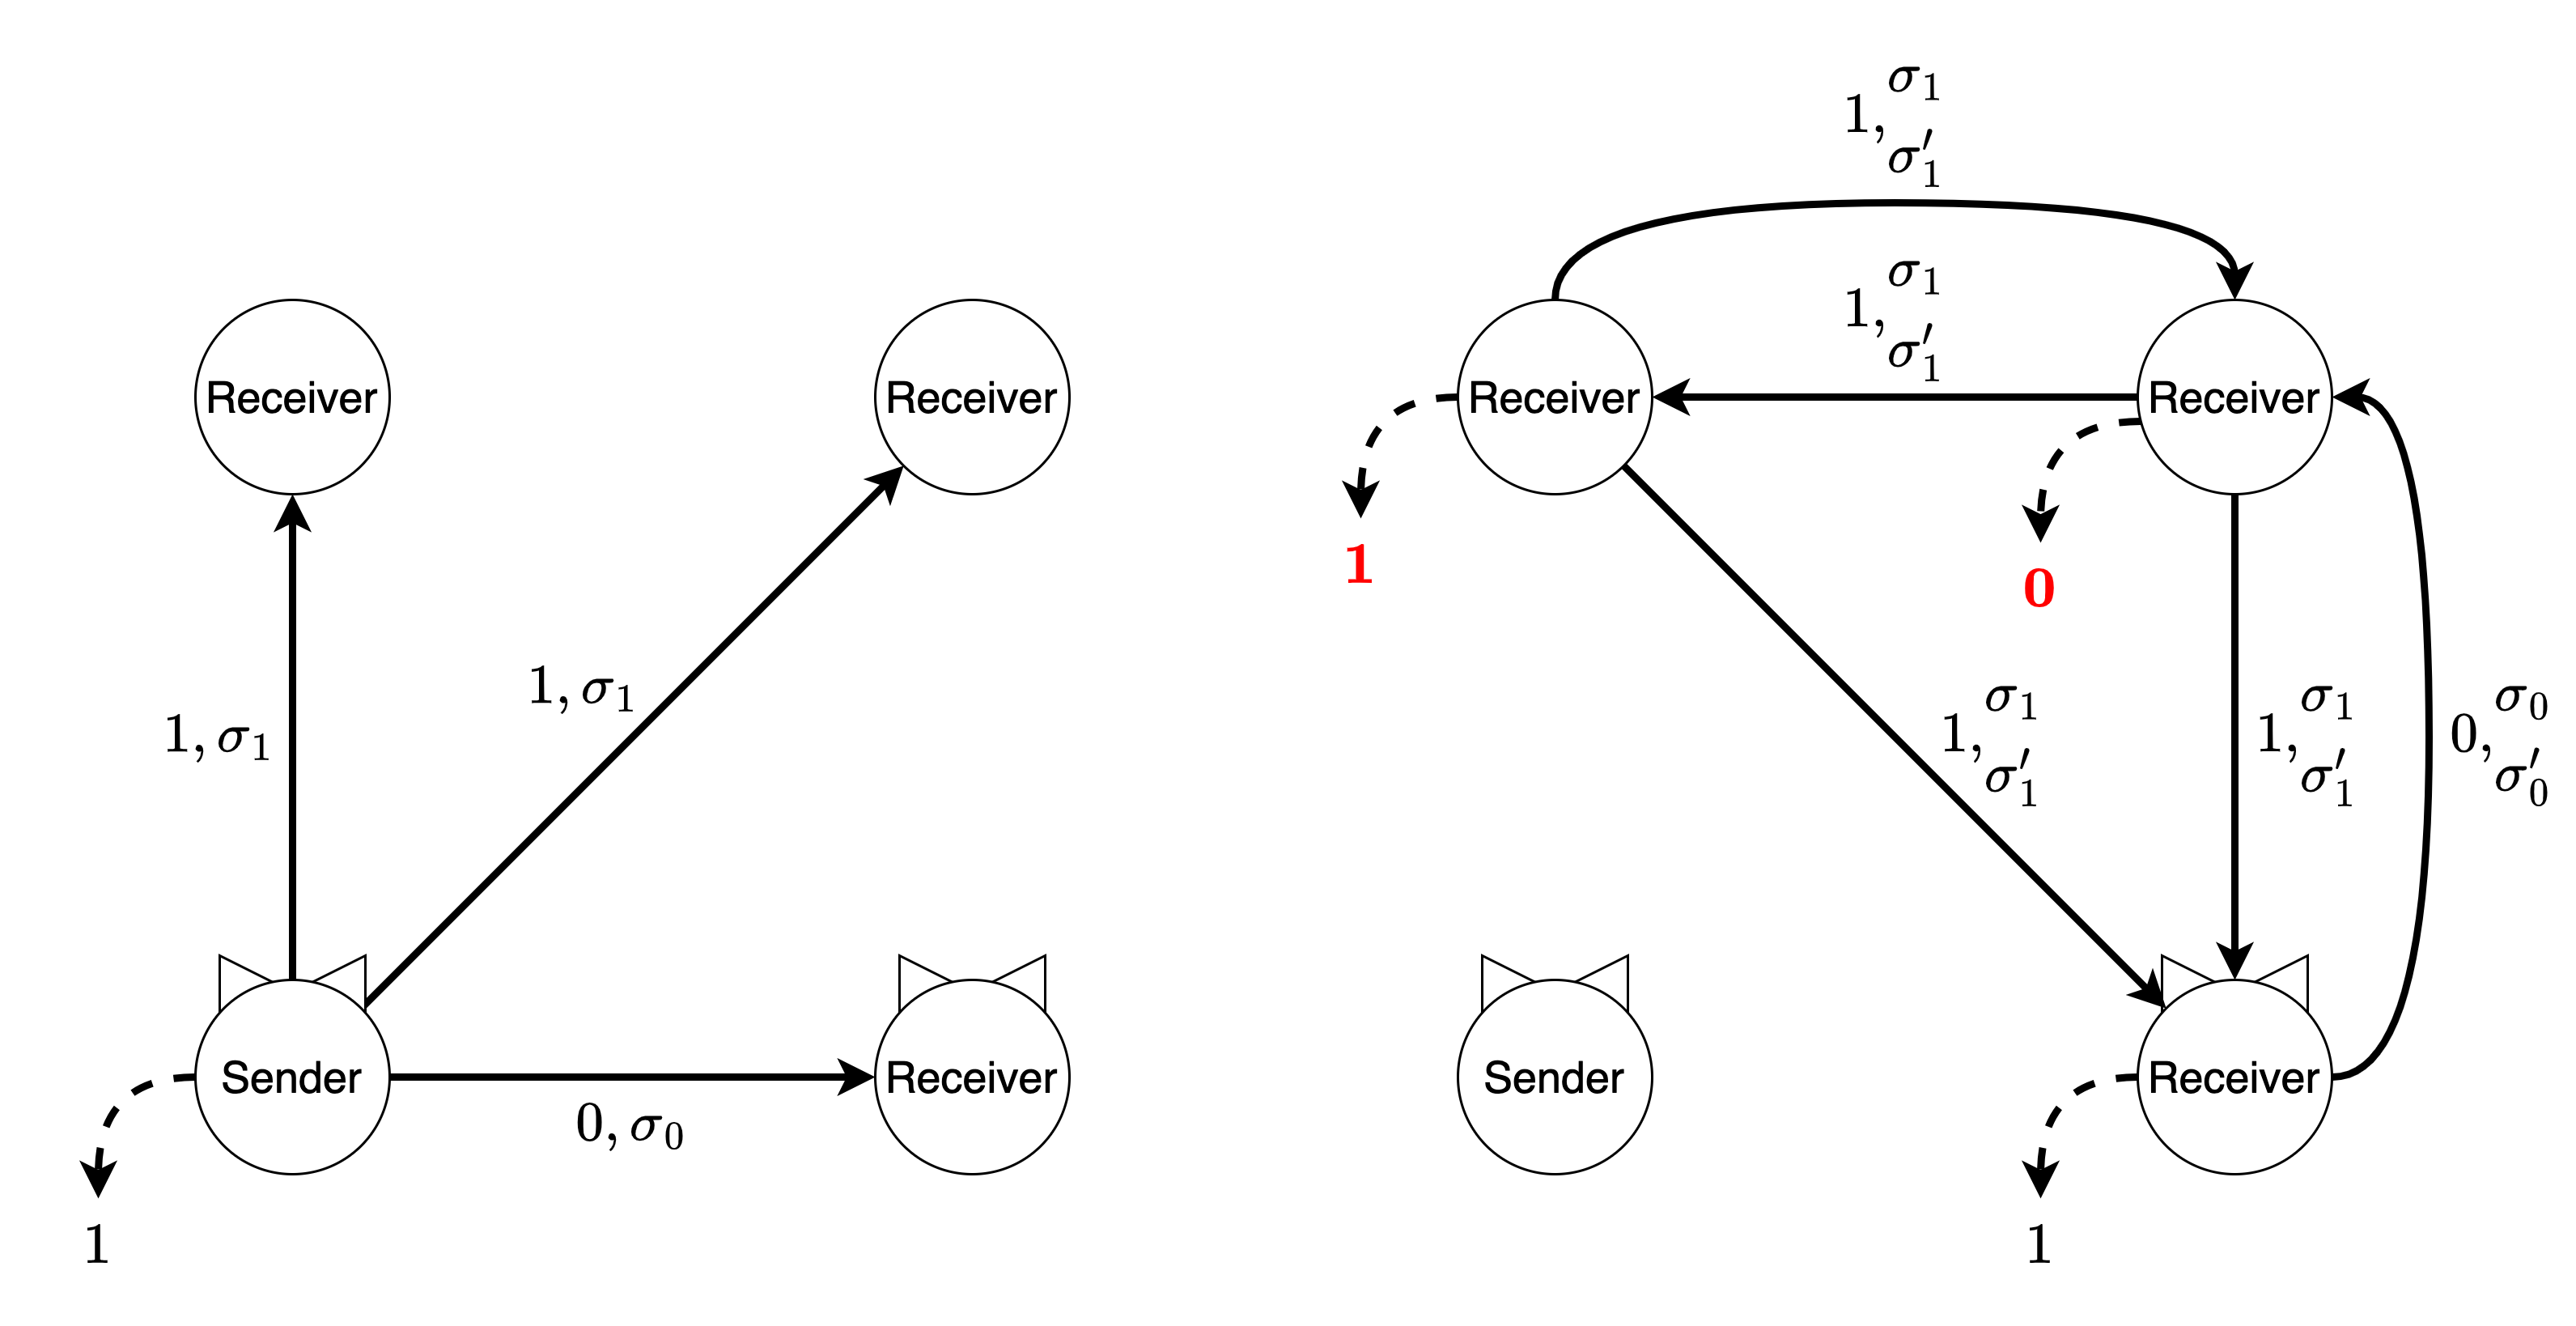
\includegraphics[width=\textwidth]{6.3.png}
            \caption{Иллюстрация атаки на свойство безопасности при наличии нечестного отправителя и 
                нечестного участника для $n = 4$}
            \label{fig:6.3}
        \end{figure}
        
        Таким образом, построена атака, позволяющая заставить каких-то честных участников вернуть ноль, а
        других --- единицу.
        
        \Answer{при наличии двух нечестных участников протокол \textit{не обладает} свойством безопасности.}
        
    \item В п. 1 показано, что при наличии одного нечестного участника свойство валидности выполнено. Покажем, 
        что это свойство сохраняется и при наличии двух нечестных участников. Отметим, что возвращаемое
        значение нечестных участников никак не учитывается, поэтому игнорирование неправильной подписи
        (при подмене бита другим нечестным участником) ни на что не влияет. Если нечестный участник (или оба
        сразу) отправляют подмененный бит честному, то последний просто игнорирует эти биты при принятии
        решения: отправка неправильного бита не приводит к нарушению свойства валидности. Если нечестный
        участник не отправил бит кому-либо, то это так же никак не влияет на принятие решения. При этом
        следует иметь в виду, что каждый честный участник уже имеет у себя бит от отправителя с правильной
        подписью, то есть возвращает в случае чего он именно его, так как не может получить от остальных
        честных участников другие биты.
        
        \Answer{при наличии не более двух нечестных игроков свойство валидности \textit{имеет место}.}
    
    \item Пусть, как и в п. 3, нечестными будут отправитель и один участник. Также положим, что существуют
        еще по меньшей мере два честных участника. Рассмотрим следующую атаку (рис. \ref{fig:6.5}):
        отправитель пересылает единицу с правильной подписью только нечестному участнику и возвращает
        после этого единицу. Затем нечестный участник (уже на втором шаге) отправляет единицу с правильной
        подписью одному из честных участников (в общем случае --- некоторому собственному подмножеству
        $\mathcal{V}$ множества $\mathcal{H}$ честных участников). После этого, данный участник возвращает 
        единицу. Более никаких передач не осуществляется согласно протоколу (шагов передачи всего два). 
        При этом другой честный участник (а в общем случае все участники из подмножества 
        $\mathcal{H} \setminus \mathcal{V}$), который не получил ничего ни от кого, ничего в итоге не 
        возвращает, что обозначает прямое нарушение свойства всеобщности.
        
        \begin{figure}[h!]
            \centering
            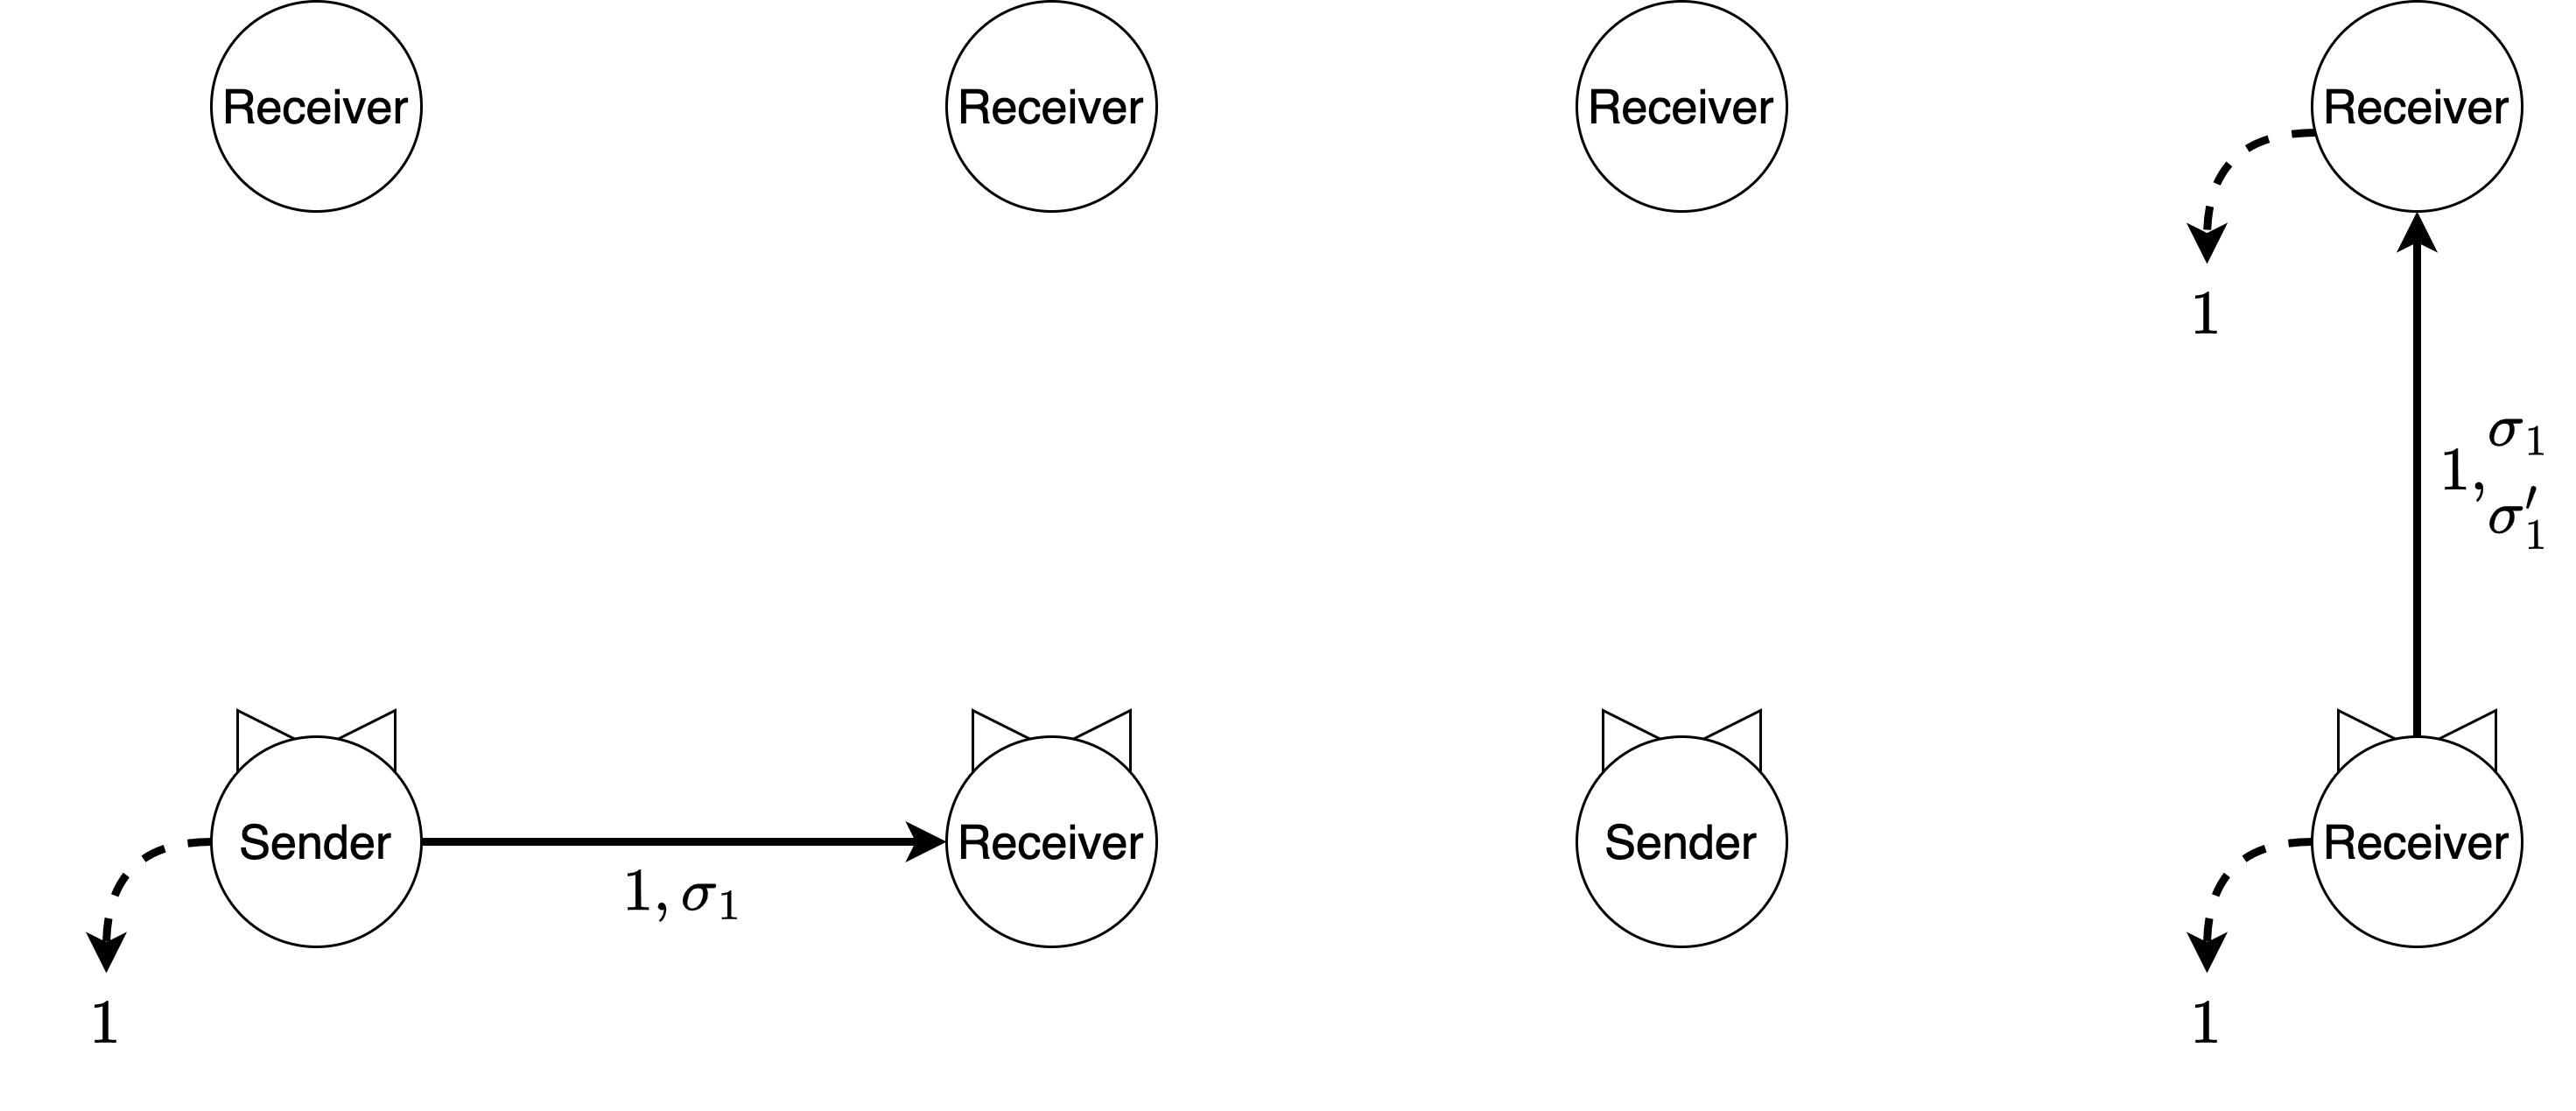
\includegraphics[width=\textwidth]{6.5.png}
            \caption{Иллюстрация атаки на свойство всеобщности при наличии нечестного отправителя и 
                нечестного участника для $n = 4$}
            \label{fig:6.5}
        \end{figure}
        
        Таким образом, при наличии как минимум двух участников протокол уже не может обладать свойством
        всеобщности. Рассмотрим теперь ситуацию с одним нечестным участником.
        
        Случай первый --- нечестный отправитель. Если участникам отправлены разные биты, то они так или
        иначе что-либо вернут, а значит свойство всеобщности выполняется --- если хотя бы один честный
        участник возвращает бит, то все честные участники тоже в том случае что-либо возвращают. Если
        какому-либо участнику бит не отправлен, то он все равно получает информацию от остальных и что-либо
        возвращает --- свойство всеобщности вновь выполнено.
        
        Второй случай --- нечестный участник, но не отправитель. Его возвращаемое значение в учет не
        берется. Но он не может заставить честного участника не вернуть хотя бы что-то, так как это
        возможно только тогда, когда этот участник \textit{вообще ничего} не получил или получил бит
        отправителя с неправильной подписью, но все участники получают бит от отправителя с валидной
        подписью, а значит что-либо да вернут. То есть свойство всеобщности вновь выполнено.
        
        \Answer{свойство всеобщности \textit{соблюдается} при наличии \underline{не более одного} нечестного 
            участника, но \underline{как минимум при двух} нечестных участниках возможна атака, 
            \textit{нарушающаяя} его.}
\end{enumerate}

\mysection{Задание 7}

\begin{enumerate}
    \item \Answer{да, так как $1 \land b = b$, то есть результат вычисления попросту равен биту Бориса.}
    
    \item \Answer{нет, так как $0 \land b = 0$, то есть каким бы ни был бит Бориса, результат будет равняться
        нулю, и Анна не сможет по нему достоверно определить бит Бориса.
    }
    
    \item \Answer{суть атаки в следующем: на ключах $K_L^0$ и $K_R^1$ зашифровывается не 0, а 1, т.е.
        $c_{01} = E_{K_L^0}\left(E_{K_R^1}(\mathbf{1})\right)$. Борис корректно расшифрует $c_{00}$ 
        (получит 0) или $c_{01}$ (получит 1). Получив от Бориса бит $b$, Анна сделает вывод, что у Бориса 
        был изначально бит $b$. Отметим, что в остальном Анна не отклоняется от протокола.
        
        Борис не сможет уличить Анну в атаке, так как для него все получаемые значения выглядят ровно
        так же, как и в <<обычном>> случае: значения $c_{ij}$, $i, j \in \{0, 1\}$ являются неотличимыми
        от случайных значениями (при использовании стойкого шифра). Это объясняется случайным и независимым
        выбором ключей шифрования. В частности, Борис не может вычислительно различить значения 
        $E_{K_L^0}\left(E_{K_R^1}(\mathbf{1})\right)$ (при атаке) и 
        $E_{K_L^0}\left(E_{K_R^1}(\mathbf{0})\right)$ (атаки нет).
    }
\end{enumerate}

\mysection{Задание 8}

\begin{enumerate}
    \item Пусть Анна сгенерировала свои доли $r_a, r_b, r_c$, а Борис --- две свои $s_a, s_b$. Задача:
        вычислить $s_c$ (Борис это значение у себя оставляет и никуда не отдает). Так как требуется 
        построить тройку Бивера, то $r_c \oplus s_c = (r_a \oplus s_a) \land (r_b \oplus s_b)$. 
        Значит требуется вычислить следующую функцию: $f = (r_a \oplus s_a) \land (r_b \oplus s_b) \oplus r_c$.
        
        Вычисление производится более чем очевидным способом (прямо как в задаче 7): Анна генерирует
        10 ключей (по два для каждой из 5 переменных), зашифровывает все значения таблицы истинности
        и передает в случайном порядке их Борису, а также и свои нужные ключи. Далее Борис при помощи
        (2, 4)-забывающей передачи получает у Анны ключи, соответствующие его значениям $s_a, s_b$.
        
        После этого, Борис расшифровывает значения и верно расшифрованное будет как раз искомым
        значением $s_c$. Передавать его Анне не потребуется.
        
        Корректность выработки следует из построения функции $f$. Стойкость неформально обосновывается
        тем фактом, что функция $f$ является равновероятной, а значит $\Pr{r_j = 0 | s_c = 0} =
        \Pr{r_j = 1 | s_c = 0} = \Pr{r_j = 0 | s_c = 1} = \Pr{r_j = 1 | s_c = 1} = \frac{1}{2}$, 
        $j \in \{a, b, c\}$. То есть Борис не может по полученному значению достоверно восстановить
        биты Анны.
        
    \item Анна генерирует значения $f$ для своих $r_1, r_b, r_c$, а также для всех 4 вариантов комбинаций
        $s_a, s_b$ битов Бориса. После этого Борис при помощи (1, 4)-забывающей передачи получает то
        значение, которое соответствует его конкретным значениям $s_a, s_b$.
    
    \item Рассмотрим следующий протокол\footnotemark[1]. Анна имеет у себя значения 
        $m_1, ..., m_{2 ^ l} \in \{0, 1\}$. Борис хочет получить значение $m_I$, где $I \in \{1, ..., 2 ^ l\}$.
        
        Анна заготавливает $2l$ ключей (каждый вырабатывается случайно и равновероятно из $\{0, 1\} ^ \lambda$):
        \begin{equation}
            \left(K_1^0, K_1^1\right), \left(K_2^0, K_2^1\right), ..., \left(K_l^0, K_l^1\right).
        \end{equation}
        
        Обозначим через $i[j]$ $j$-й бит $l$-битного числа $i$ (т.е. $j \in \{1, ..., l\}$). 
        
        Для каждого $1 \leq i \leq 2 ^ l$ Анна вычисляет значение 
        $c_i = m_i \oplus \bigoplus_{j = 1}^{l} F\left( K_j^{i[j]}, i \right)$.
        
        Далее наступает шаг использования (1, 2)-забывающей передачи. Борис знает номер $I$ сообщения,
        которое хочет получить, и поочередно получает ключи $K_j^{I[j]}$ для всех $j \in \{1, ..., l\}$ 
        (то есть используется как раз $l$ вызовов протокола (1, 2)-забывающей передачи $\lambda$-битных
        сообщений).
        
        После этого Анна передает Борису все $c_i$ для $i \in \{1, ..., 2 ^ l\}$, а Борис восстанавливает
        искомое сообщение:
        \begin{equation}
            m_I = c_I \oplus \bigoplus_{j = 1}^{l} F\left( K_j^{I[j]}, I \right).
        \end{equation}
    
        \footnotetext[1]{Идея протокола была взята из статьи: Naor, M., Pinkas, B. (1999). Oblivious 
            transfer and polynomial evaluation. Proceedings of the Thirty-First Annual ACM Symposium 
            on Theory of Computing - STOC ’99. doi:10.1145/301250.301312}
\end{enumerate}

\mysection{Задание 9}

\begin{enumerate}
    \item Будем считать, что при возможных значениях $m$ оно достаточно быстро находится по известным $g$ и 
        $g ^ m$ (то есть задача дискретного логарифма для таких значений $m$ решается за приемлемое время).
        
        Тогда алгоритм $\texttt{Dec}(sk, (u, v))$ описывается следующей последовательностью действий:
        \begin{itemize}
            \item вычисляется значение $w = \frac{u ^ c}{v ^ a} = g ^ {m(c - ab)}$ (так как $c \ne ab$, 
                показатель может быть равен нулю только если $m = 0$);
            
            \item перебираются различные кандидаты $\tilde{m}$ для $m$, пока не будет найдено такое, что
                $g ^ {\tilde{m}(c - ab)} = w$. Это и будет расшифрованным сообщением.
        \end{itemize}
        
    \item Отметим, что значение $r$ никак не участвует в расшифровании, поэтому алгоритм 
        $\texttt{Add}(pk, ct_1, ct_2)$ строится достаточно очевидным способом:
        \begin{equation}
        \begin{split}
            & \texttt{Add}(pk, ct, ct') = (u_{sum}, v_{sum}) \\
            & u_{sum} = u \cdot u' = g ^ {m + a r} g ^ {m' + a r'} = 
                g ^ {(m + m') + a (r + r')} \\
            & v_{sum} = v \cdot v' = g ^ {m b + c r} g ^ {m' b + c r'} = 
                g ^ {(m + m') b + c (r + r')}
        \end{split}
        \end{equation}
        
    \item Запишем значения $u, u', v, v'$ в аддитивной нотации (все-таки аддитивные группы):
        \begin{equation}
        \begin{split}
            u  & = (m + r a) g \\
            v  & = (m b + r c) g \\
            u' & = (m' + r' a') h \\
            v' & = (m' b' + r' c') h
        \end{split}
        \end{equation}
        
        В силу билинейности отношения спаривания $e$ верно:
        \begin{equation}
        \begin{split}
            \alpha_1 & = (m + r a)(m' + r' a') \\
            \alpha_2 & = (m + r a)(m' b' + r' c') \\
            \alpha_3 & = (m b + r c)(m' + r' a') \\
            \alpha_4 & = (m b + r c)(m' b' + r' c')
        \end{split}
        \end{equation}
        
        Тогда запишем:
        \begin{equation}
        \begin{split}
            m m' & = C_1 \alpha_1 + C_2 \alpha_2 + C_3 \alpha_3 + C_4 \alpha_4,
        \end{split}
        \end{equation}
        для некоторых $C_j$, $j \in \{1, ..., 4\}$.
        
        Теперь подставим значения для $\alpha_j$, $j \in \{1, ..., 4\}$ и раскроем скобки:
        \begin{equation}
        \begin{split}
            m m' & = C_1 (m + r a)(m' + r' a') + C_2 (m + r a)(m' b' + r' c') + \\
            & + C_3 (m b + r c)(m' + r' a') + C_4 (m b + r c)(m' b' + r' c') = \\
            & = m m' (C_1 + C_2 b' + C_3 b + C_4 b b') + m r' (C_1 a' + C_2 c' + C_3 b a' + C_4 b c') + \\
            & + m' r (C_1 a + C_2 a b' + C_3 c + C_4 c b') + r r' (C_1 a a' + C_2 a c' + C_3 c a' + C_4 c c').
        \end{split}
        \label{eq:mm-equality}
        \end{equation}
        
        По равенству несложно составить следующую СЛАУ относительно $C_j$, $j \in \{1, ..., 4\}$:
        \begin{equation}
            \left\{\begin{array}{lclclclcl}
                C_1      & + & C_2 b'   & + & C_3 b    & + & C_4 b b' & = & 1 \\
                C_1 a'   & + & C_2 c'   & + & C_3 b a' & + & C_4 b c' & = & 0 \\
                C_1 a    & + & C_2 a b' & + & C_3 c    & + & C_4 c b' & = & 0 \\
                C_1 a a' & + & C_2 a c' & + & C_3 c a' & + & C_4 c c' & = & 0
            \end{array}
            \right.
        \label{eq:slae}
        \end{equation}
        
        Несложно заметить, что при условии, что $C_j$, $j \in \{1, ..., 4\}$ являются решениями
        данной системы, равенство (\ref{eq:mm-equality}) выполняется. Осталось доказать, что данная
        система совместна. Воспользуемся теоремой Кронекера-Капелли.
        
        Приведем (расширенную) матрицу системы к каноническому виду:
        \begin{equation}
        \begin{split}
            & 
            \begin{array}{||cccc|c||}
                1    & b'   & b    & b b' & 1 \\
                a'   & c'   & b a' & b c' & 0 \\
                a    & a b' & c    & c b' & 0 \\
                a a' & a c' & c a' & c c' & 0
            \end{array}
            \sim
            \begin{array}{||cccc|c||}
                1  & b'   & b    & b b' & 1 \\
                a' & c'   & b a' & b c' & 0 \\
                a  & a b' & c    & c b' & 0 \\
                0  & 0    & a'   & c'   & 0
            \end{array}
            \sim \\ \sim\ &
            \begin{array}{||cccc|c||}
                1 & b'         & b      & b b'           & 1   \\
                0 & c' - a' b' & 0      & b (c' - a' b') & -a' \\
                0 & 0          & c - ab & b' (c - ab)    & -a  \\
                0 & 0          & a'     & c'             & 0
            \end{array}
            \sim
            \begin{array}{||cccc|c||}
                1 & b' & b  & b b' & 1                      \\
                0 & 1  & 0  & b    & \frac{-a'}{c' - a' b'} \\
                0 & 0  & 1  & b'   & \frac{-a}{c - ab}      \\
                0 & 0  & a' & c'   & 0
            \end{array}
            \sim \\ \sim\ &
            \begin{array}{||cccc|c||}
                1 & b' & b & b b'       & 1                      \\
                0 & 1  & 0 & b          & \frac{-a'}{c' - a' b'} \\
                0 & 0  & 1 & b'         & \frac{-a}{c - ab}      \\
                0 & 0  & 0 & c' - a' b' & \frac{a a'}{c - ab}
            \end{array}
            \sim
            \begin{array}{||cccc|c||}
                1 & b' & b & b b' & 1                      \\
                0 & 1  & 0 & b    & \frac{-a'}{c' - a' b'} \\
                0 & 0  & 1 & b'   & \frac{-a}{c - ab}      \\
                0 & 0  & 0 & 1    & \frac{a a'}{(c - ab)(c' - a' b')}
            \end{array}
        \end{split}
        \end{equation}
        
        Заметим, что ранг матрицы системы равен рангу расширенной матрицы системы, а значит,
        по теореме Кронекера-Капелли система уравнений (\ref{eq:slae}) совместна. Отсюда следует,
        что найдутся такие $C_j$, $j \in \{1, ..., 4\}$, что выполнено равенство (\ref{eq:mm-equality}),
        а значит $mm'$ выражается линейной комбинацией $\alpha_j$, $j \in \{1, ..., 4\}$.
        
    \item Для восстановления открытого текста будем использовать свойство билинейности спаривания $e$.
        Сперва заметим, что (вновь используем аддитивную нотацию):
        \begin{equation}
        \begin{split}
            w_1 ^ {c c'} & = e\left((m + r a) g, (m' + r' a') h\right) ^ {c c'} = 
                e\left((m c + r a c) g, (m' c' + r' a' c') h\right) \\
            w_4 ^ {a a'} & = e\left((m b + r c) g, (m' b' + r' c') h\right) ^ {a a'} =
                e\left((m a b + r a c) g, (m' a' b' + r' a' c') h\right)
        \end{split}
        \label{eq:raised-pairings}
        \end{equation}
        
        При этом в силу того, что $e(a, b) = e(a, b) ^ {(-1) (-1)} = e(-a, -b)$, верно следующее:
        \begin{equation}
            w_4 ^ {a a'} = e\left(-(m a b + r a c) g, -(m' a' b' + r' a' c') h\right)
        \label{eq:switched-sign}
        \end{equation}
        
        Вновь воспользуемся свойством билинейности $e$, а также (\ref{eq:raised-pairings}) и 
        (\ref{eq:switched-sign}):
        \begin{equation}
        \begin{split}
            w_1 ^ {c c'} w_4 ^ {a a'} = e\left((m (c - a b) g, m' (c' - a' b') h\right) =
                e(g, h) ^ {m m' (c - a b)(c' - a' b')},
        \end{split}
        \end{equation}
        где $e(g, h)$ --- генератор группы $\mathbb{G}_T$.
        
        Так как $m$ и $m'$ лежат в малых интервалах, то можно перебором их произведение и найти.
\end{enumerate}

\pagebreak
\mysection{Приложение А. Исходный код для задачи 3.3}

\begin{lstlisting}[language=python]
def get_max_2_power(x):
    power = 0
    
    while x % 2 == 0:
        x //= 2
        power += 1
        
    return 2 ** power


def is_power_of_two(x):
    result = False
    
    while x % 2 == 0:
        x //= 2
    
    return x == 1
    
    
def get_path(k):
    long_hops  = 0
    short_hops = 0
    path       = []
    
    position   = k - 1
    
    while position != 0:
        path.append(position)
    
        if position % 2 != 0 or is_power_of_two(position):
            position -= 1
            short_hops += 1
        else:
            position -= get_max_2_power(position)
            long_hops += 1
    
    return long_hops, short_hops, path
\end{lstlisting}

\end{document}
